\documentclass{article}
\usepackage[portuguese]{babel}
\usepackage[utf8]{inputenc}
\usepackage{amsmath}
\usepackage{amssymb}
\usepackage{graphicx}
\usepackage{caption}
\usepackage{float}
\usepackage{subcaption}
\usepackage{pdflscape}
\usepackage{multirow}
\usepackage[table,xcdraw]{xcolor}

\author{Cláudio Ferreira Carneiro - RA 263796}
\title{EFC 2}
\begin{document}
    \maketitle
    \pagenumbering{gobble}
    \newpage
    \pagenumbering{arabic}
    \section[]{Parte II – Classificação binária com redes MLP e SVMs}
    O código referente às atividades se encontra no repositório:
    
    https://github.com/carneirofc/IA006.git\linebreak
    \subsection*{a)} Antes da inicialização do treinamento,
    os dados de entrada foram redimensionados utilizando o \textit{standard scaler},
    tendo a média removida e escalado à variância unitária, equação \ref{eq:std_scaler}.
    A classe representada por $-1$ passará a ser representada por $0$ a fim de utilizar a
    função de custo \textit{Binary Cross-Entropy} no treinamento do modelo. A figura \ref{fig:out_data_scaled}
    apresenta o histograma das saídas (classes) do \textit{dataset} de treinamento.
    \begin{align}
        z &= (x - \mu) / \sigma
        \label{eq:std_scaler}
    \end{align}
    A figura \ref{fig:inp_data_scaled} apresenta os dados de treinamento de entrada originais e 
    escalados pelo \textit{standard scaler}. Nota-se que não ocorreram mudanças significativas
    no \textit{dataset}.
    \begin{figure}[H]
        \centering
        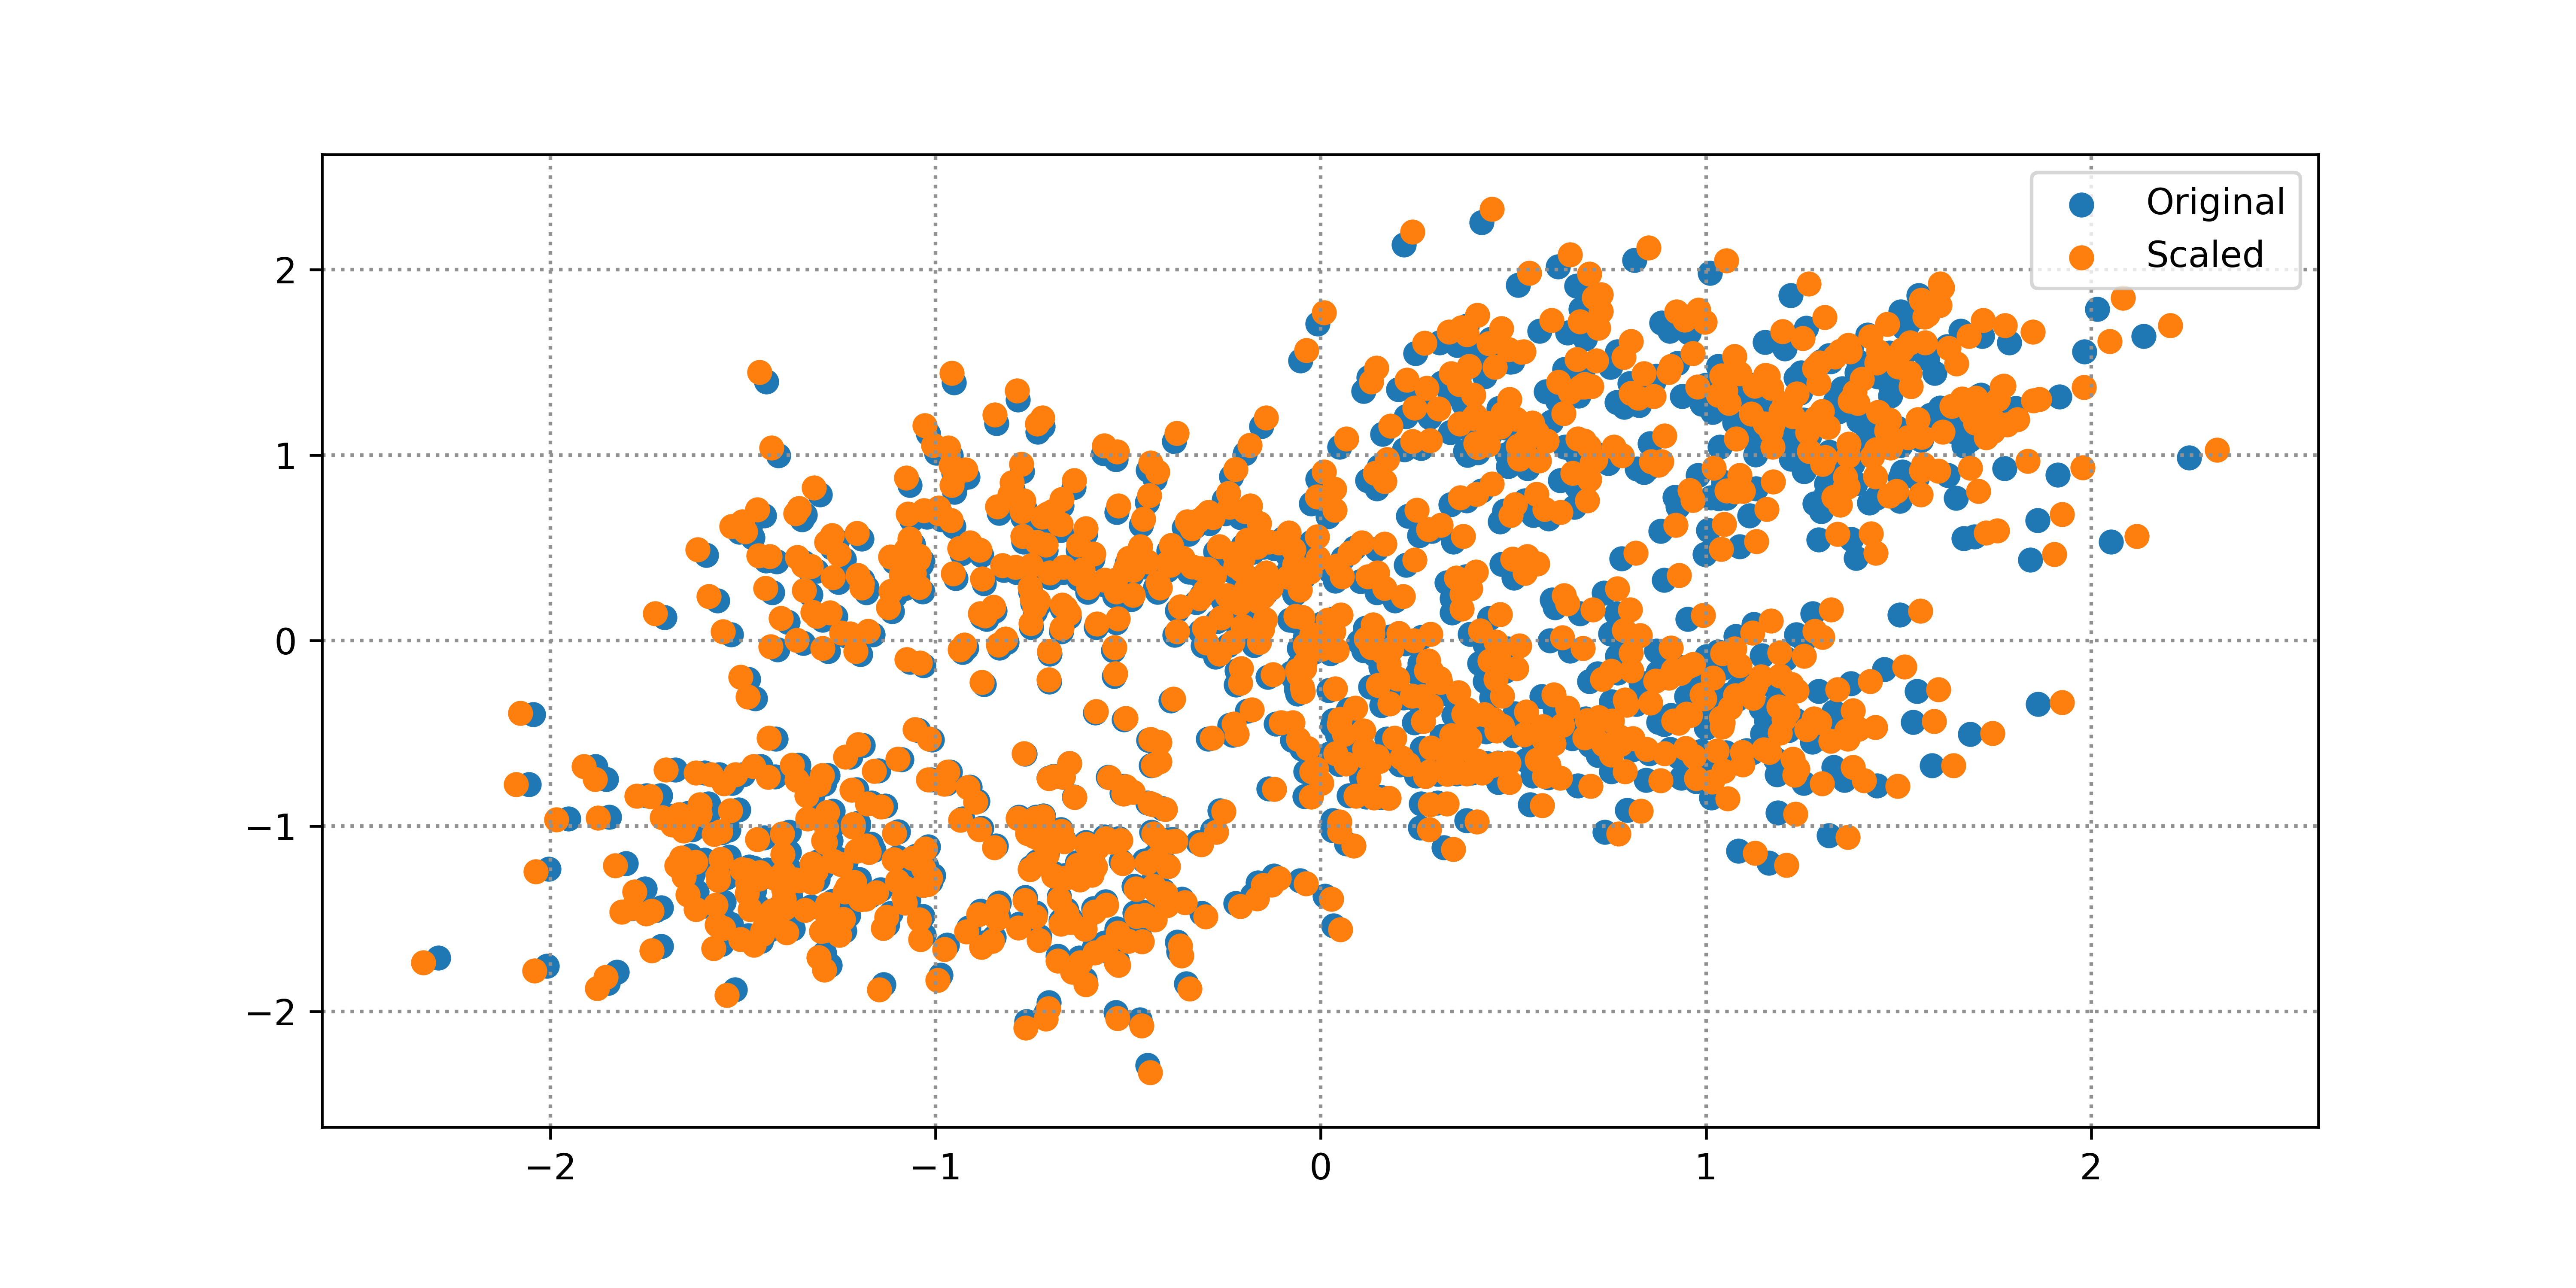
\includegraphics[width=\linewidth]{mlp_inp_scaled.png}   
        \caption{\textit{Dataset} de treinamento, atributos de entrada
            originais e escalados.}
        \label{fig:inp_data_scaled}
    \end{figure}
    
    \begin{figure}[H]
        \centering
        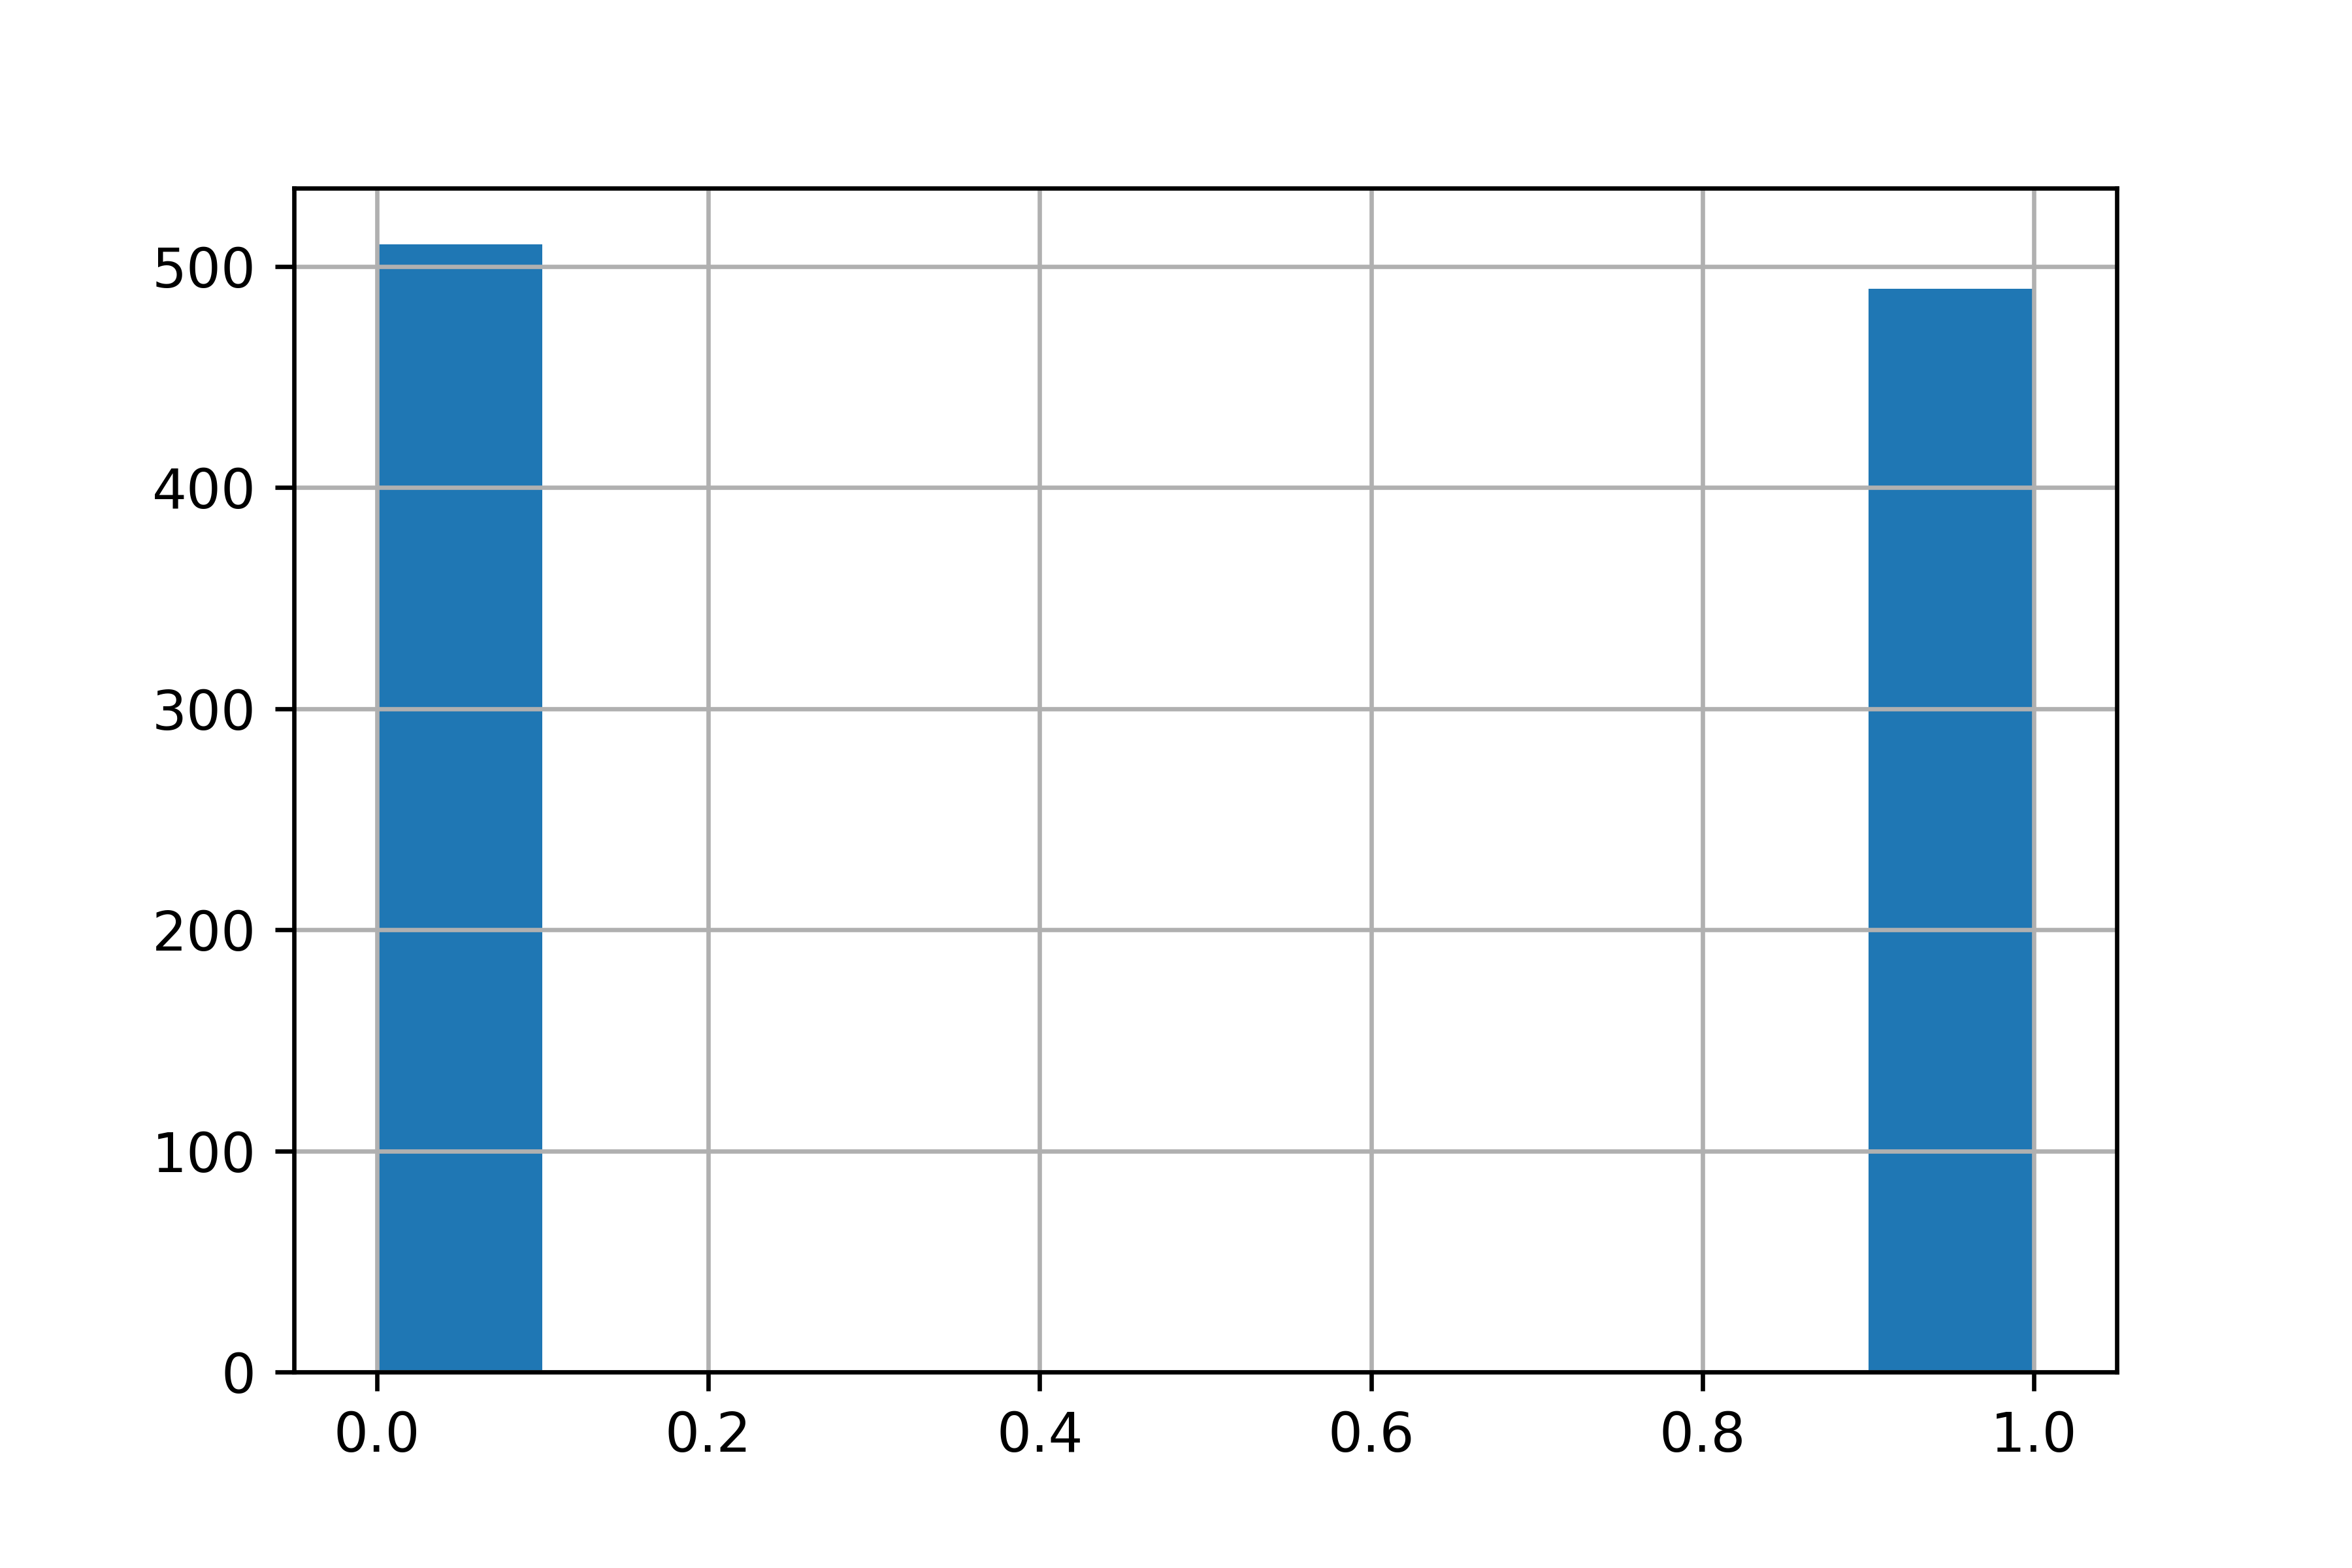
\includegraphics[width=\linewidth]{mlp_out_scaled.png}   
        \caption{\textit{Dataset} de treinamento, classes $0$ e $1$.}
        \label{fig:out_data_scaled}
    \end{figure}
    A MPL foi definida como uma rede de $35$ neurônios na camada intermediária, utilizando
    como função de ativação a \textit{ReLU}. Na camada de saída apenas um neurônio é utilizado,
    cuja função de ativação é a \textit{sigmoid}, equação \ref{eq:sigmoid}.
    O processo de treinamento da MPL utilizou o \textit{RMSprop} como algoritmo de treinamento.
    \begin{align}
        y(x) &= \frac{1}{1 + \exp^{-x}}
        \label{eq:sigmoid}
    \end{align}
    O processo de treinamento foi definido com duração de $1000$ épocas com critérios de 
    parada prematura. Os dados de entrada foram embaralhados e apresentados
    em \textit{batch} com $10$ amostras.
    Como critério de parada prematura é utilizada a variação do erro de validação. A melhor configuração
    da MLP durante o treinamento é restaurada por \textit{snapshots} da configuração de pesos de menor custo
    nos dados de validação.

    Quando o erro de validação da época não superar o limiar especificado ($0.001$) por $patience=200$ épocas,
    o treinamento é finalizado.
    
    A MLP foi treinada por $200$ épocas, onde o treinamento foi interrompido pela
    parada prematura, com custo de treinamento $0.3225$ e custo de validação
    $0.3459$. A figura \ref{fig:mlp_training} apresenta o histórico do erro de treinamento
    e validação. Os pesos atribuídos à MLP são provenientes da época $146$, onde o custo de validação
    é $0.3391$.

    \begin{figure}[H]
        \centering
        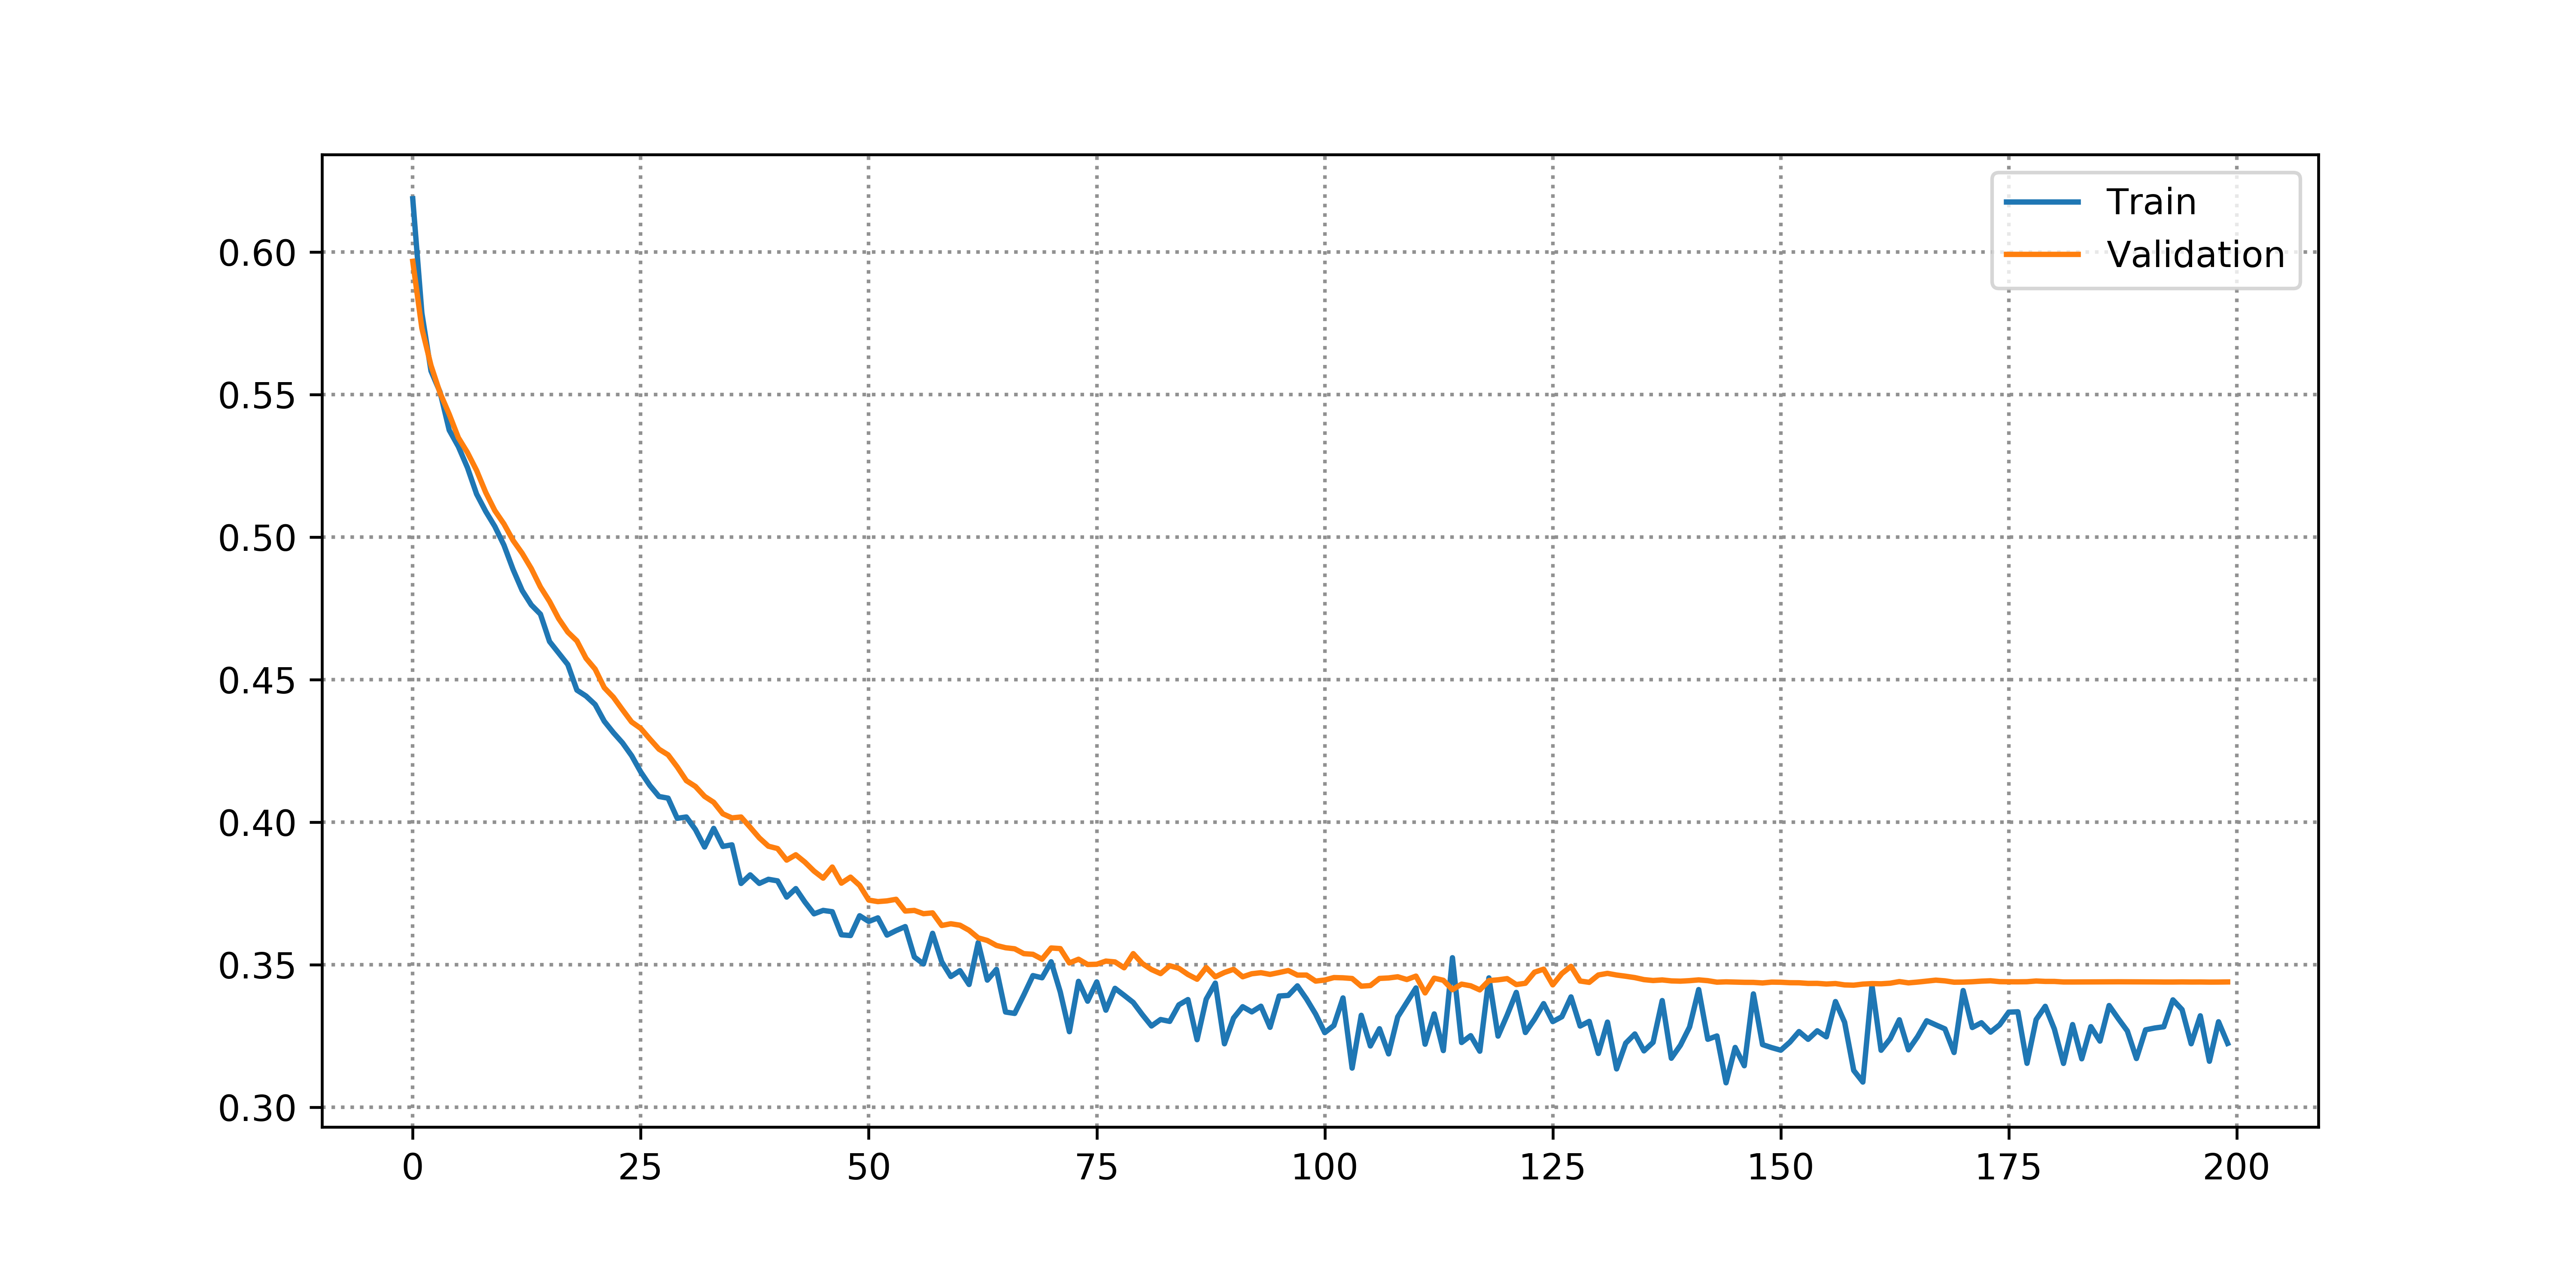
\includegraphics[width=\linewidth]{mlp_training.png}   
        \caption{Histórico de erro no processo de treinamento.}
        \label{fig:mlp_training}
    \end{figure}
   
    A curva ROC da MLP é vista na figura \ref{fig:mlp_roc}, com pontuação de $\approx0.9261$ para os dados de validação.
    \begin{figure}[H]
        \centering
        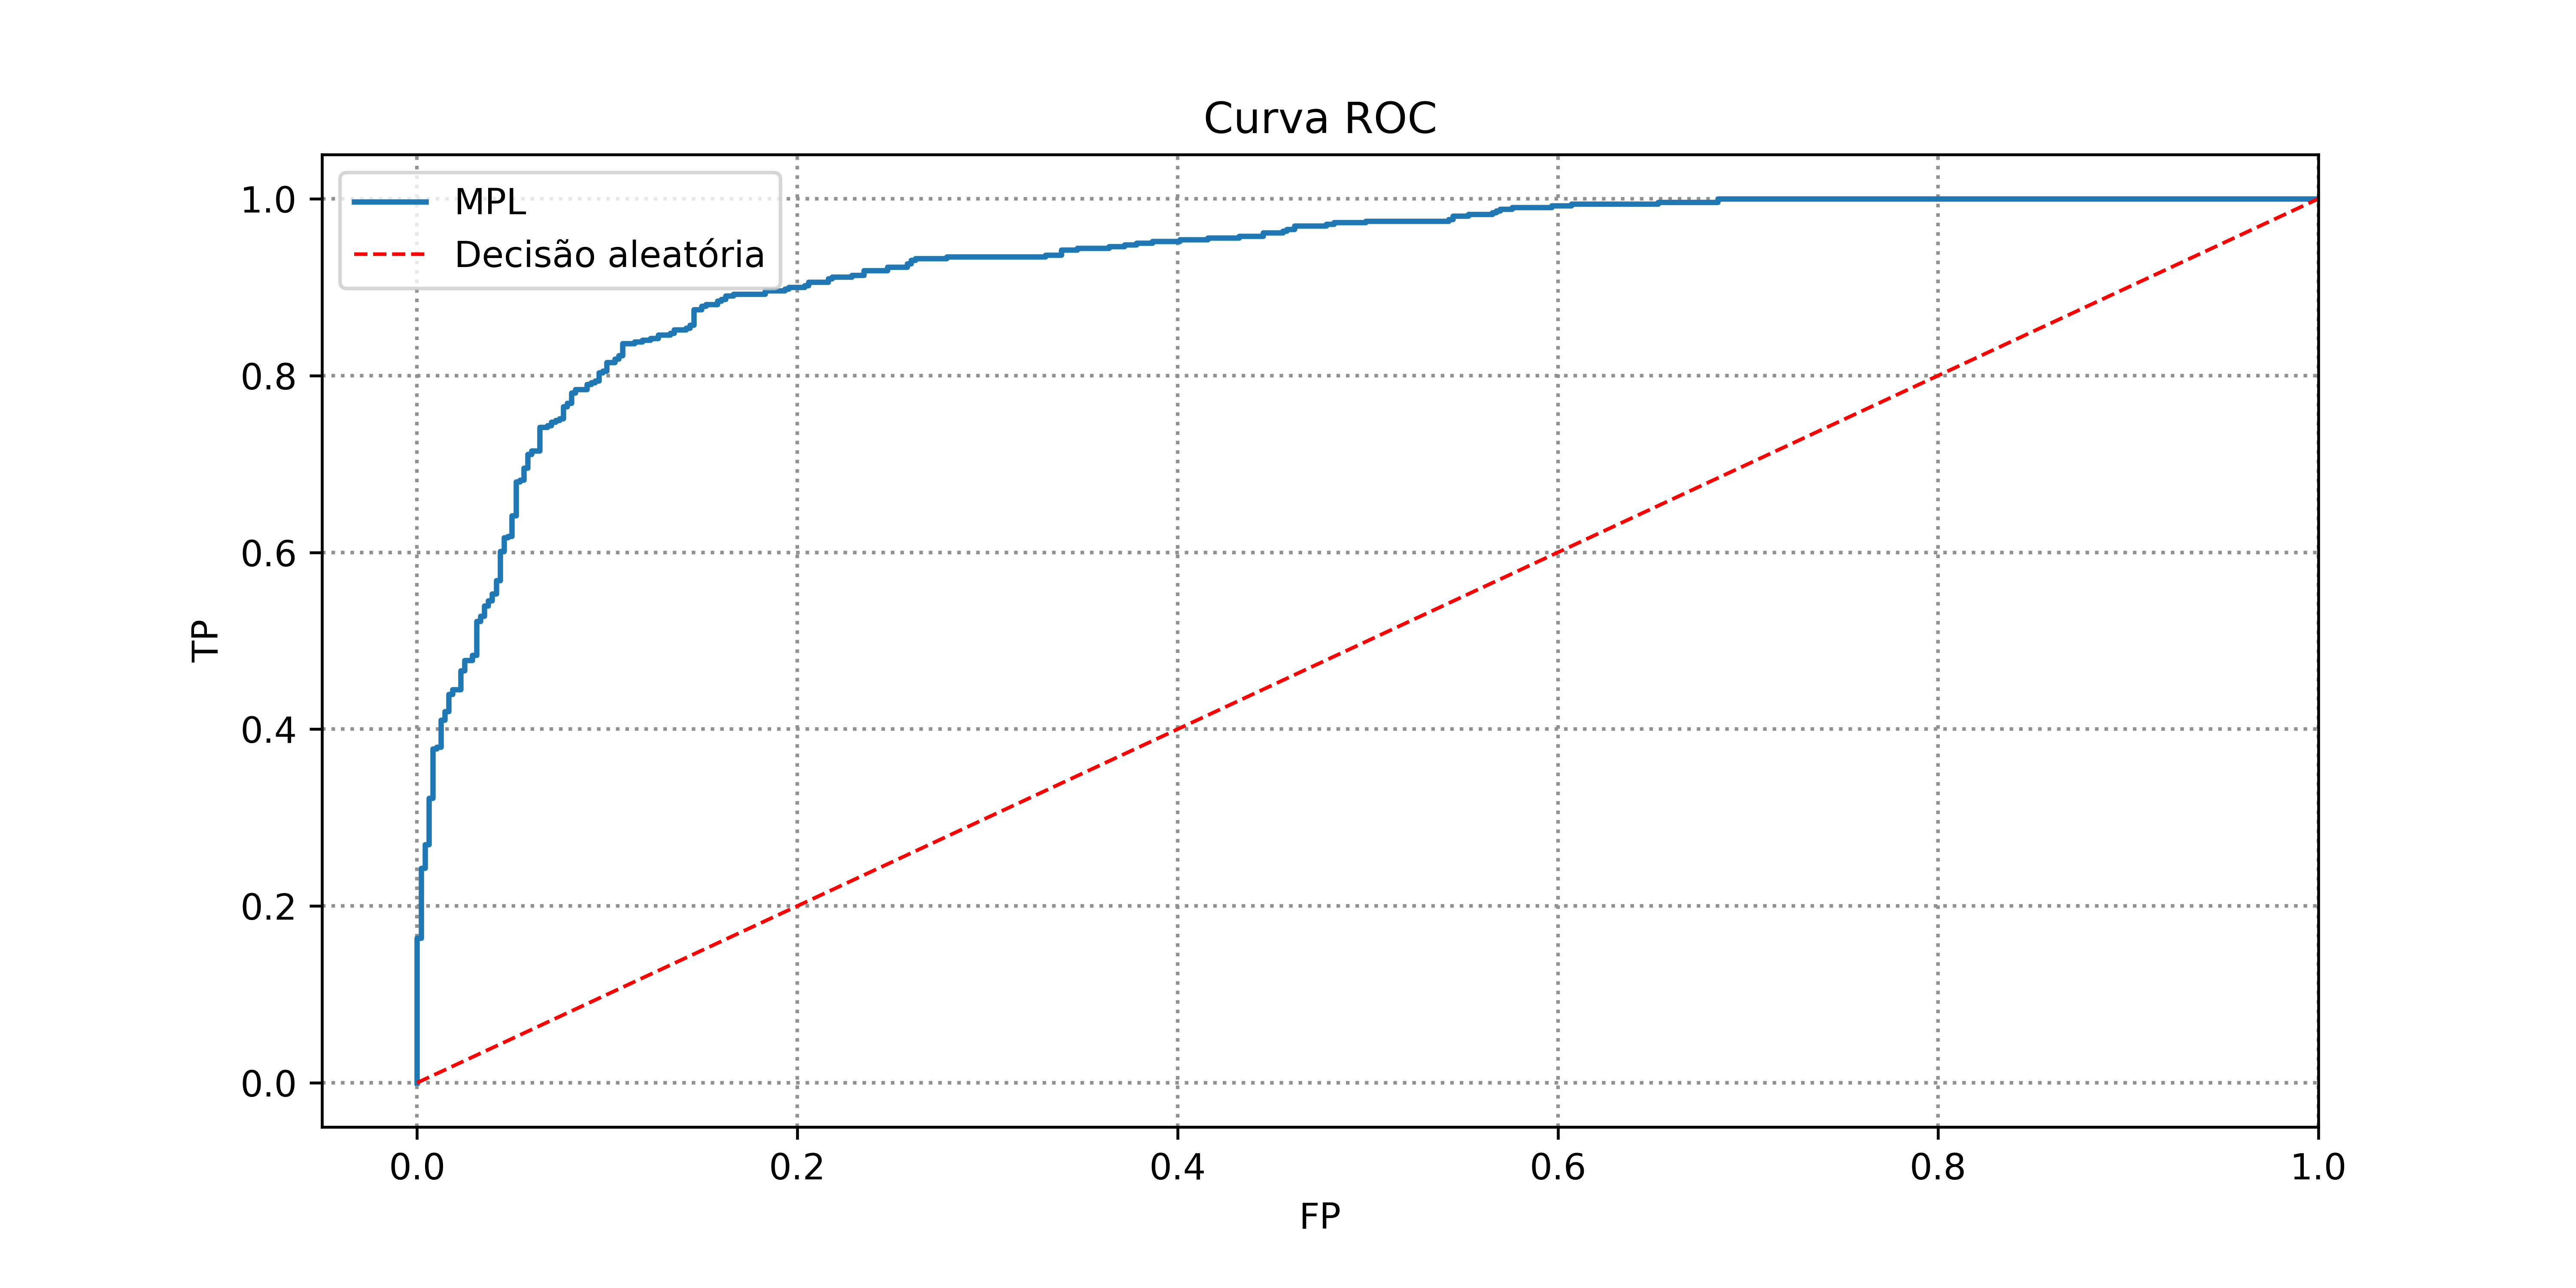
\includegraphics[width=\linewidth]{mlp_roc.png}   
        \caption{Curva ROC da MLP para os dados de validação.}
        \label{fig:mlp_roc}
    \end{figure}

    \subsection*{b)}
    A região de decisão se assemelha à região ótima porém é visível que ainda existem padrões
    a serem capturados pela MPL.
    \begin{figure}[H]
        \centering
        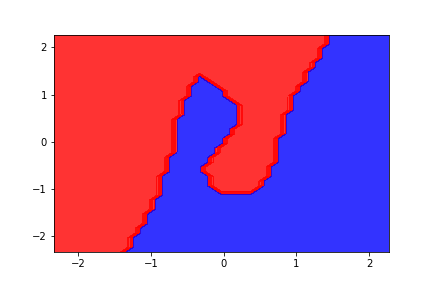
\includegraphics[width=\linewidth]{mpl_decision.png}   
        \caption{Regiões de decisão.}
        \label{fig:mpl_decision}
    \end{figure}

    \subsection*{c)}
    A MPL obteve uma acurácia de $87\%$ como é visto na tabela \ref{tbl:mpl_test}.
    \begin{table}[H]
        \begin{tabular}{c|c|c|c|c|}
        \cline{2-5}
                                        & \textbf{Precision} & \textbf{Recall} & \textbf{f1-score} & \textbf{support} \\ \hline
        \multicolumn{1}{|c|}{Classe -1}    & 0.86               & 0.88            & 0.87              & 499              \\ \hline
        \multicolumn{1}{|c|}{Classe 1}     & 0.88               & 0.86            & 0.87              & 501              \\ \hline
        \multicolumn{1}{|c|}{}             &                    &                 &                   &                  \\ \hline
        \multicolumn{1}{|c|}{accuracy}     &                    &                 & 0.87              & 1000             \\ \hline
        \multicolumn{1}{|c|}{macro avg}    & 0.87               & 0.87            & 0.87              & 1000             \\ \hline
        \multicolumn{1}{|c|}{weighted avg} & 0.87               & 0.87            & 0.87              & 1000             \\ \hline
        \end{tabular}
        \caption{Classificação do \textit{dataset} de teste, MLP.}
        \label{tbl:mpl_test}
    \end{table}

    \subsection*{d)}
    Utilizando as configurações de treinamento citadas anteriormente,
    $7$ MLPs foram treinadas com camadas escondidas de $5, 15, 25, 35, 45, 55$ e $65$ neurônios.
    A as curvas ROC dos classificadores são apresentadas na figura \ref{fig:mpl_roc_multi}. 
    
    As redes com $5$ e $15$ neurônios apresentaram desempenho inferior às demais configurações, um forte indicador de que o modelo
    não é suficientemente flexível para a classificação dos dados.
    
    \begin{figure}[H]
        \centering
        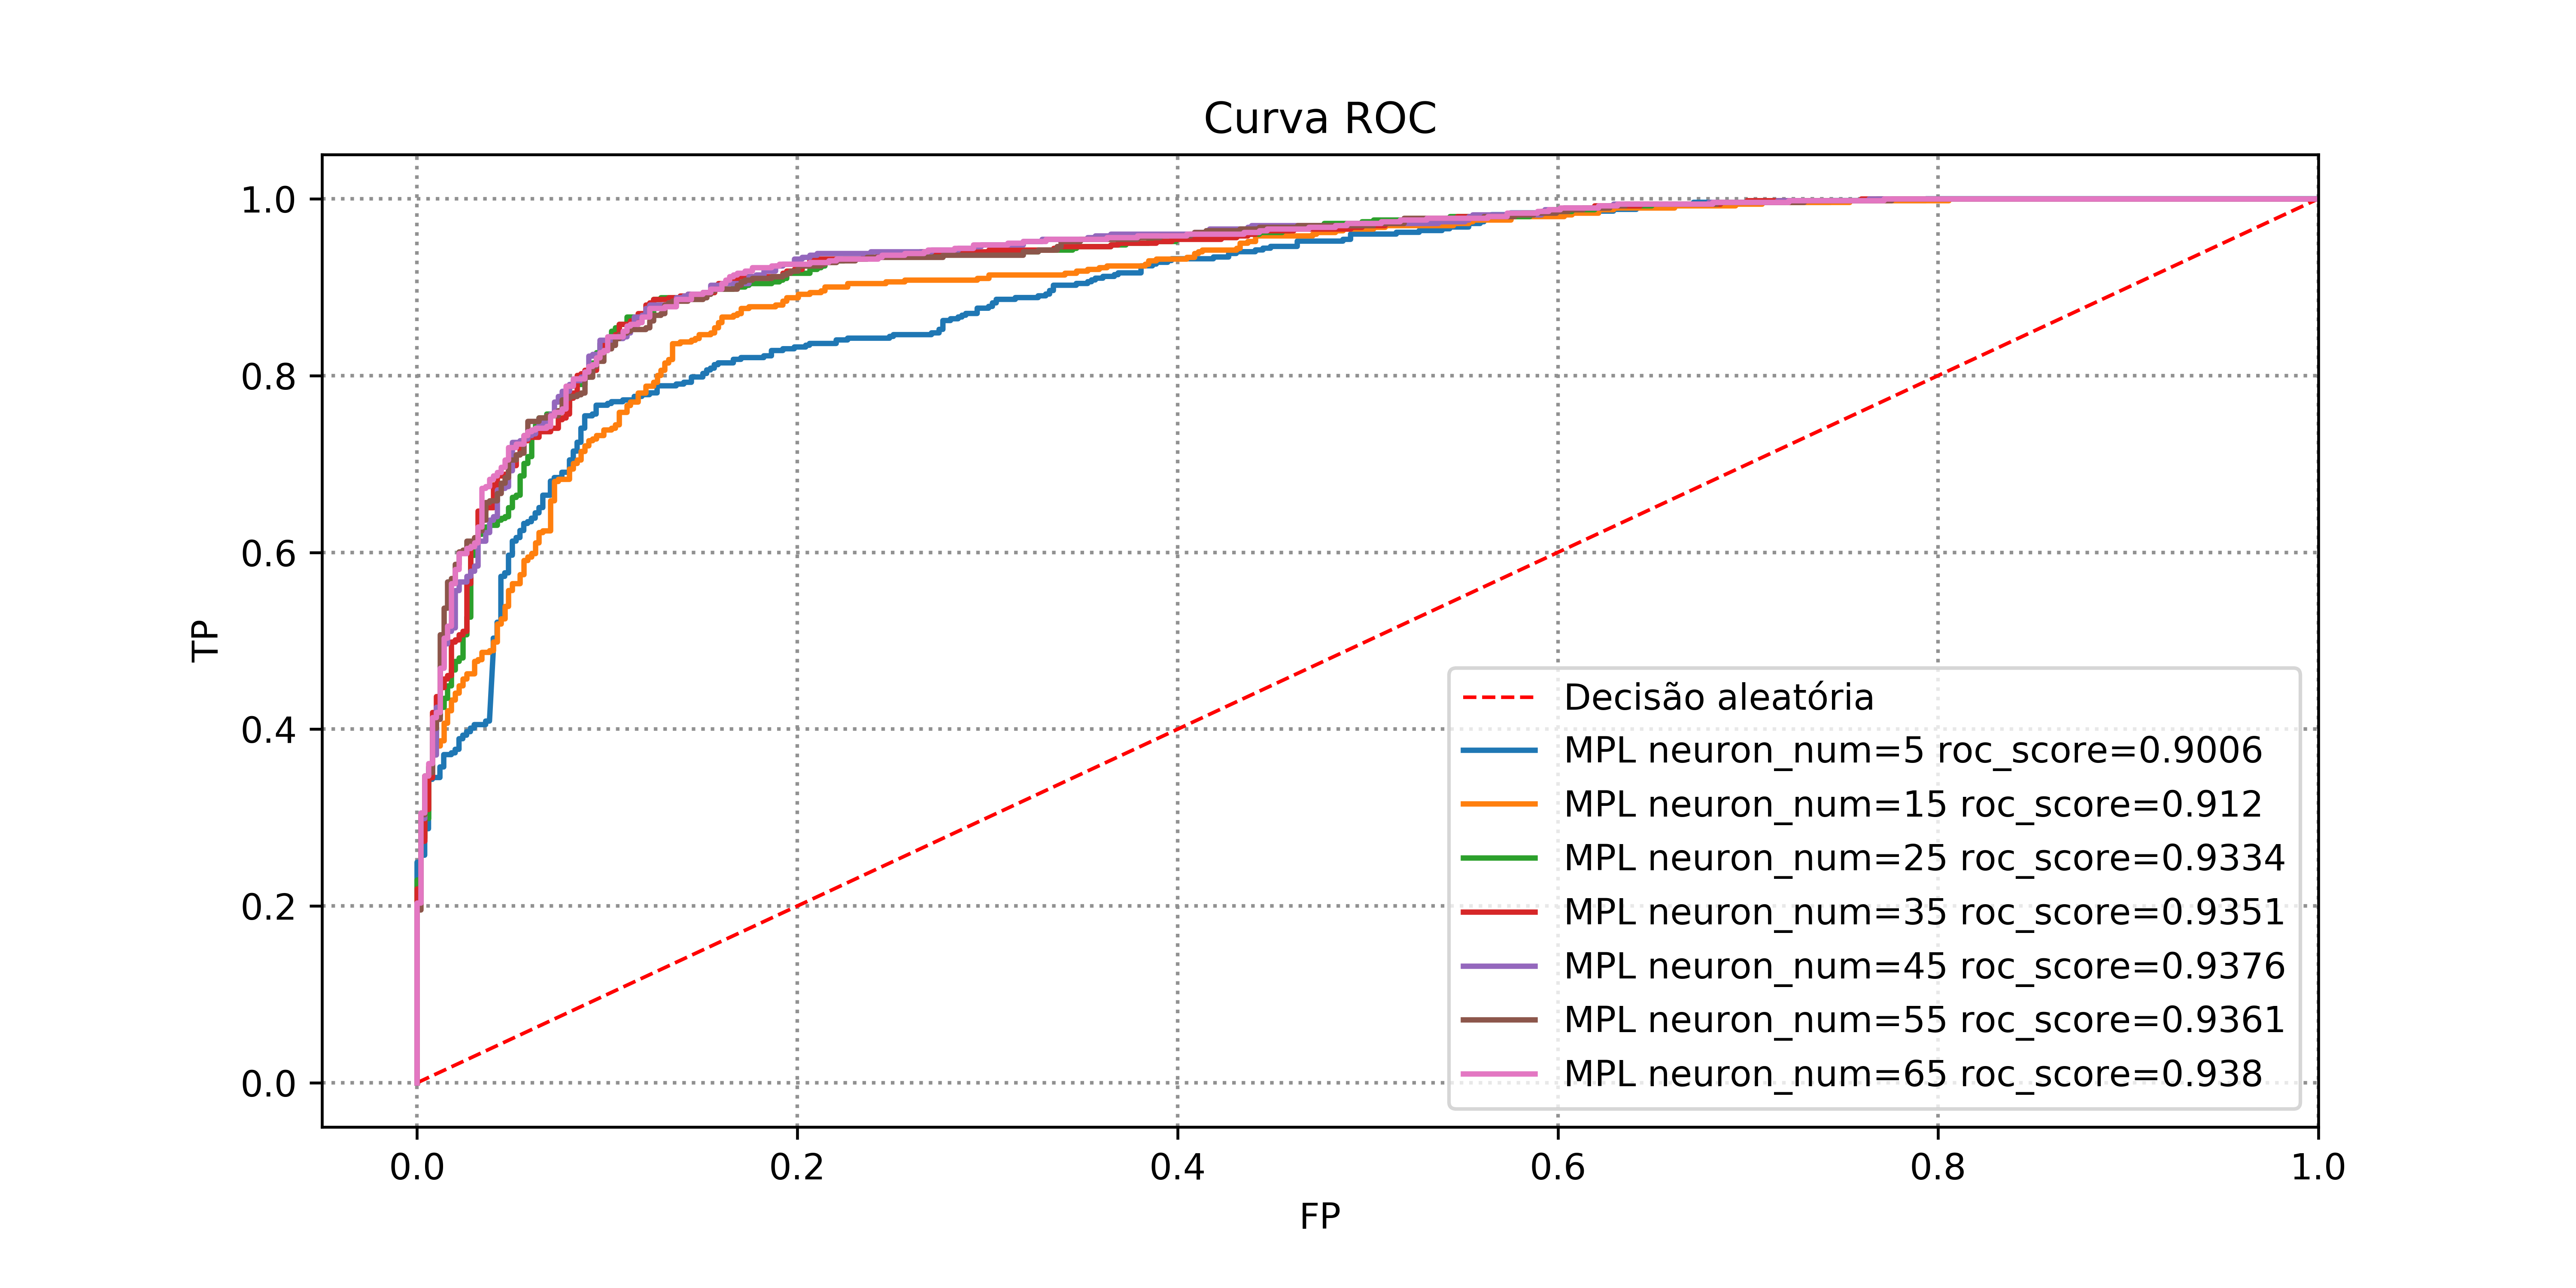
\includegraphics[width=\linewidth]{mlp_roc_multi.png}   
        \caption{Curvas ROC dos classificadores MLP.}
        \label{fig:mpl_roc_multi}
    \end{figure}

    Conforme os resultados da classificação do \textit{dataset} apresentado na tabela \ref{tbl:mlp_multi}, o ganho no desempenho
    de classificação conforme o número de neurônio não é linear. As MLPs de $25, 35, 45,55$ e $65$ apresentaram performance similar,
    tanto em sua acurácia quanto na $f1-score$.
    
    \begin{table}[H]
        \begin{tabular}{c|c|c|c|c|}
        \cline{2-5}
                                & \textbf{macro avg precision} & \textbf{macro avg recall} & \textbf{macro avg f1-score} & \textbf{accuracy} \\ \hline
        \multicolumn{1}{|c|}{5}  & 0.7975081828740365           & 0.7817711270845084        & 0.7790265816831282          & 0.782             \\ \hline
        \multicolumn{1}{|c|}{15} & 0.8324343163756176           & 0.8281153124612499        & 0.8274589111453519          & 0.828             \\ \hline
        \multicolumn{1}{|c|}{25} & 0.8750660095053688           & 0.8750135000540002        & 0.8749968749218731          & 0.875             \\ \hline
        \multicolumn{1}{|c|}{35} & 0.8717637345901665           & 0.8710454841819367        & 0.8709430859008823          & 0.871             \\ \hline
        \multicolumn{1}{|c|}{45} & 0.8723651286157541           & 0.8720314881259525        & 0.8719749070817879          & 0.872             \\ \hline
        \multicolumn{1}{|c|}{55} & 0.8682107087827426           & 0.8670574682298728        & 0.8669029722667825          & 0.867             \\ \hline
        \multicolumn{1}{|c|}{65} & 0.8705731075673273           & 0.8700394801579207        & 0.869957866348697           & 0.87              \\ \hline
        \end{tabular}
        \caption{Resultado da classificação das MLPs.}
        \label{tbl:mlp_multi}
    \end{table}
    
    \subsection*{e)}
    Vetores suporte e regiões de decisão da SVM de $C=1$ e kernel RBF. 
    \begin{figure}[H]
        \centering
        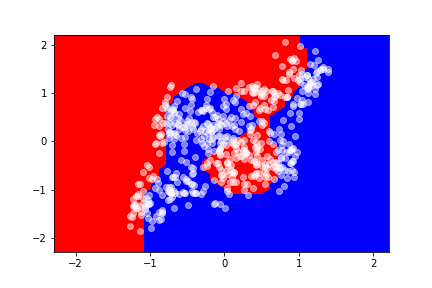
\includegraphics[width=\linewidth]{svm_decision.png}   
        \caption{Regiões de decisão SVM.}
        \label{fig:svm_decision}
    \end{figure}

    \subsection*{f)}
    Com o uso da SVM é obtida uma acurácia de $87\%$ conforme a tabela \ref{tbl:svm_test}.
    \begin{table}[H]
        \begin{tabular}{c|c|c|c|c|}
        \cline{2-5}
                                        & \textbf{Precision} & \textbf{Recall} & \textbf{f1-score} & \textbf{support} \\ \hline
        \multicolumn{1}{|c|}{Classe -1}    & 0.86               & 0.87            & 0.87              & 499              \\ \hline
        \multicolumn{1}{|c|}{Classe 1}     & 0.87               & 0.86            & 0.87              & 501              \\ \hline
        \multicolumn{1}{|c|}{}             &                    &                 &                   &                  \\ \hline
        \multicolumn{1}{|c|}{accuracy}     &                    &                 & 0.87              & 1000             \\ \hline
        \multicolumn{1}{|c|}{macro avg}    & 0.87               & 0.87            & 0.87              & 1000             \\ \hline
        \multicolumn{1}{|c|}{weighted avg} & 0.87               & 0.87            & 0.87              & 1000             \\ \hline
        \end{tabular}
        \caption{Classificação do \textit{dataset} de teste, SVM.}
        \label{tbl:svm_test}
    \end{table} 
    \subsection*{g)}
    As figuras \ref{fig:svm_decision_linear} e \ref{fig:svm_decision_poly} apresentam
    as regiões de decisão de SVMs com kernel linear e polinomial respectivamente. Nota-se
    que a escolha do kernel possui um impacto significativo no desempenho da SVM. Conforme as
    regiões de decisão obtidas, os kernels não possuem a flexibilidade exigida pelo problema.
    
    \begin{figure}[H]
        \centering
        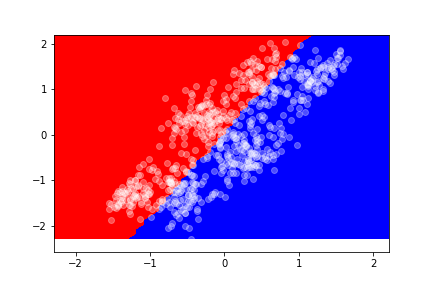
\includegraphics[width=\linewidth]{svm_decision_linear.png}   
        \caption{Regiões de decisão, SVM com kernel linear.}
        \label{fig:svm_decision_linear}
    \end{figure}
    
    \begin{figure}[H]
        \begin{subfigure}{.5\textwidth}
            \centering
                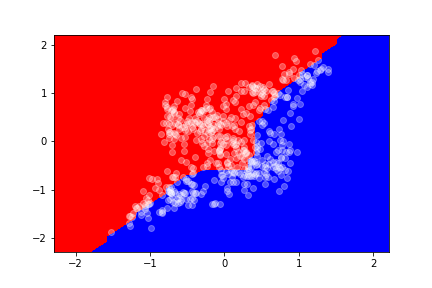
\includegraphics[width=\linewidth]{svm_decision_poly.png}   
            \caption{Polinômio de grau 3}
        \end{subfigure}
        \begin{subfigure}{.5\textwidth}
            \centering
                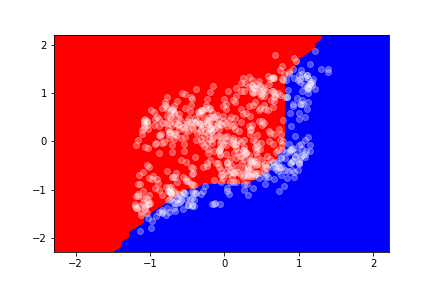
\includegraphics[width=\linewidth]{svm_decision_poly_9.png}   
            \caption{Polinômio de grau 9}
        \end{subfigure}
        \caption{Regiões de decisão SVM, com kernel polinomial de grau $3$ e $9$.}
        \label{fig:svm_decision_poly}
    \end{figure}

    A figura \ref{fig:svm_decision_C} apresenta as regiões de decisão conforme o parâmetro
    $C$ é modificado. Para valores baixos de $C$, a SVM tende a classificar incorretamente
    maiores quantidades de amostras.
    
    \begin{figure}[H]
        \begin{subfigure}{.3\textwidth}
            \centering
            \includegraphics[width=\linewidth]{{svm_decision_0.1}.png}   
        \end{subfigure}
        \begin{subfigure}{.3\textwidth}
            \centering
            \includegraphics[width=\linewidth]{{svm_decision_0.2}.png}   
        \end{subfigure}
        \begin{subfigure}{.3\textwidth}
            \centering
            \includegraphics[width=\linewidth]{{svm_decision_0.3}.png}   
        \end{subfigure}
        \begin{subfigure}{.3\textwidth}
            \centering
            \includegraphics[width=\linewidth]{{svm_decision_0.4}.png}   
        \end{subfigure}
        \begin{subfigure}{.3\textwidth}
            \centering
            \includegraphics[width=\linewidth]{{svm_decision_0.5}.png}   
        \end{subfigure}
        \begin{subfigure}{.3\textwidth}
            \centering
            \includegraphics[width=\linewidth]{{svm_decision_0.6}.png}   
        \end{subfigure}
        \begin{subfigure}{.3\textwidth}
            \centering
            \includegraphics[width=\linewidth]{{svm_decision_0.6}.png}   
        \end{subfigure}
        \begin{subfigure}{.3\textwidth}
            \centering
            \includegraphics[width=\linewidth]{{svm_decision_0.7}.png}   
        \end{subfigure}
        \begin{subfigure}{.3\textwidth}
            \centering
            \includegraphics[width=\linewidth]{{svm_decision_0.8}.png}   
        \end{subfigure}
        \begin{subfigure}{.3\textwidth}
            \centering
            \includegraphics[width=\linewidth]{{svm_decision_0.9}.png}   
        \end{subfigure}
        \begin{subfigure}{.3\textwidth}
            \centering
            \includegraphics[width=\linewidth]{{svm_decision_1.0}.png}   
        \end{subfigure}
        \begin{subfigure}{.3\textwidth}
            \centering
            \includegraphics[width=\linewidth]{{svm_decision_1.1}.png}   
        \end{subfigure}
        \begin{subfigure}{.3\textwidth}
            \centering
            \includegraphics[width=\linewidth]{{svm_decision_1.2}.png}   
        \end{subfigure}
        \begin{subfigure}{.3\textwidth}
            \centering
            \includegraphics[width=\linewidth]{{svm_decision_1.3}.png}   
        \end{subfigure}
        \begin{subfigure}{.3\textwidth}
            \centering
            \includegraphics[width=\linewidth]{{svm_decision_1.4}.png}   
        \end{subfigure}
        \begin{subfigure}{.3\textwidth}
            \centering
            \includegraphics[width=\linewidth]{{svm_decision_1.5}.png}   
        \end{subfigure}
        \begin{subfigure}{.3\textwidth}
            \centering
            \includegraphics[width=\linewidth]{{svm_decision_1.6}.png}   
        \end{subfigure}
        \begin{subfigure}{.3\textwidth}
            \centering
            \includegraphics[width=\linewidth]{{svm_decision_1.7}.png}   
        \end{subfigure}
        \begin{subfigure}{.3\textwidth}
            \centering
            \includegraphics[width=\linewidth]{{svm_decision_1.8}.png}   
        \end{subfigure}
        \begin{subfigure}{.3\textwidth}
            \centering
            \includegraphics[width=\linewidth]{{svm_decision_1.9}.png}   
        \end{subfigure}
        \begin{subfigure}{.3\textwidth}
            \centering
            \includegraphics[width=\linewidth]{{svm_decision_2.0}.png}   
        \end{subfigure}
        \caption{Regiões de decisão SVM, com kernel RBF para diversos $C$.}
        \label{fig:svm_decision_C}
    \end{figure}

\end{document}